\documentclass[letterpaper, 10 pt, conference]{ieeeconf}  % Comment this line out if you need a4paper
%\documentclass[a4paper, 10pt, conference]{ieeeconf}      % Use this line for a4 paper
\IEEEoverridecommandlockouts                              % This command is only needed if
\overrideIEEEmargins                                      % Needed to meet printer requirements.

%%%%%%%%%%%%%%%%%%%%%%%%%%%%%%%%%%%%%%%%%%%%%%%%%%%%%%%%%%%%%%%%%%%%%%%%%%%%%%%%

\usepackage{amsmath}
\usepackage{amssymb}
\usepackage{graphicx}
\usepackage{rotating}
\usepackage{xcolor}

%%%%%%%%%%%%%%%%%%%%%%%%%%%%%%%%%%%%%%%%

\DeclareMathOperator*{\argmin}{arg\,min}
\DeclareMathOperator*{\argmax}{arg\,max}
\DeclareMathOperator*{\vectorize}{vec}

\newcommand{\normal}[2]{\ensuremath{\mathcal{N}\left({{#1}},{{#2}}\right)}}
\newcommand{\trans}[1]{\ensuremath{{#1}^{\mathsf{T}}}}

\newcommand{\e}{\mathbf{e}}
\newcommand{\bb}{\mathbf{k}}
\newcommand{\kL}{\mathbf{k}^L}
\newcommand{\kG}{\mathbf{k}^G}
%\newcommand{\uu^m}{\mathbf{w}}
\newcommand{\x}{\mathbf{x}}
\newcommand{\y}{\mathbf{y}}
\newcommand{\uu}{\mathbf{u}}
\newcommand{\vv}{\mathbf{v}}
\newcommand{\timestep}{s}

\newcommand{\fixme}[1]{\textbf{FIXME: {#1}}}
\newcommand{\new}[1]{\color{red} {#1}}

%%%%%%%%%%%%%%%%%%%%%%%%%%%%%%%%%%%%%%%%%%%%%%%%%%%%%%%%%%%%%%%%%%%%%%%%%%%%%%%%

\begin{filecontents}{paper.bib}
@inproceedings{wan2000unscented,
  title={The unscented Kalman filter for nonlinear estimation},
  author={Wan, Eric A and Van Der Merwe, Rudolph},
  booktitle={Adaptive Systems for Signal Processing, Communications, and Control Symposium 2000. AS-SPCC. The IEEE 2000},
  pages={153--158},
  year={2000},
  organization={Ieee}
}

@inproceedings{morelande2006reduced,
  title={Reduced sigma point filtering for partially linear models},
  author={Morelande, Mark R and Ristic, Branko},
  booktitle={2006 IEEE International Conference on Acoustics Speech and Signal Processing Proceedings},
  volume={3},
  pages={III--III},
  year={2006},
  organization={IEEE}
}

@inproceedings{padilla2010adaptive,
  title={An adaptive-covariance-rank algorithm for the unscented Kalman filter},
  author={Padilla, Lauren E and Rowley, Clarence W},
  booktitle={49th IEEE Conference on Decision and Control (CDC)},
  pages={1324--1329},
  year={2010},
  organization={IEEE}
}

@article{wang2010generating,
  title={Generating statistically correct random topologies for testing smart grid communication and control networks},
  author={Wang, Zhifang and Scaglione, Anna and Thomas, Robert J},
  journal={IEEE transactions on Smart Grid},
  volume={1},
  number={1},
  pages={28--39},
  year={2010},
  publisher={IEEE}
}

@inproceedings{hines2010topological,
  title={The topological and electrical structure of power grids},
  author={Hines, Paul and Blumsack, Seth and Sanchez, E Cotilla and Barrows, Clayton},
  booktitle={System Sciences (HICSS), 2010 43rd Hawaii International Conference on},
  pages={1--10},
  year={2010},
  organization={IEEE}
}


@article{schultz2014random,
  title={A random growth model for power grids and other spatially embedded infrastructure networks},
  author={Schultz, Paul and Heitzig, Jobst and Kurths, J{\"u}rgen},
  journal={The European Physical Journal Special Topics},
  volume={223},
  number={12},
  pages={2593--2610},
  year={2014},
  publisher={Springer}
}

@article{ghahremani2011online,
  title={Online state estimation of a synchronous generator using unscented Kalman filter from phasor measurements units},
  author={Ghahremani, Esmaeil and Kamwa, Innocent},
  journal={IEEE Transactions on Energy Conversion},
  volume={26},
  number={4},
  pages={1099--1108},
  year={2011},
  publisher={IEEE}
}

@article{ghahremani2016local,
  title={Local and wide-area pmu-based decentralized dynamic state estimation in multi-machine power systems},
  author={Ghahremani, Esmaeil and Kamwa, Innocent},
  journal={IEEE Transactions on Power Systems},
  volume={31},
  number={1},
  pages={547--562},
  year={2016},
  publisher={IEEE}
}

@article{ghahremani2011dynamic,
  title={Dynamic state estimation in power system by applying the extended Kalman filter with unknown inputs to phasor measurements},
  author={Ghahremani, Esmaeil and Kamwa, Innocent},
  journal={IEEE Transactions on Power Systems},
  volume={26},
  number={4},
  pages={2556--2566},
  year={2011},
  publisher={IEEE}
}

@article{wang2012alternative,
  title={An alternative method for power system dynamic state estimation based on unscented transform},
  author={Wang, Shaobu and Gao, Wenzhong and Meliopoulos, AP Sakis},
  journal={IEEE Transactions on Power Systems},
  volume={27},
  number={2},
  pages={942--950},
  year={2012},
  publisher={IEEE}
}

@article{qing2015decentralized,
  title={Decentralized unscented Kalman filter based on a consensus algorithm for multi-area dynamic state estimation in power systems},
  author={Qing, Xiangyun and Karimi, Hamid Reza and Niu, Yugang and Wang, Xingyu},
  journal={International Journal of Electrical Power \& Energy Systems},
  volume={65},
  pages={26--33},
  year={2015},
  publisher={Elsevier}
}

@article{rigatos2013distributed,
  title={A distributed state estimation approach to condition monitoring of nonlinear electric power systems},
  author={Rigatos, G and Siano, Q and Zervos, N},
  journal={Asian Journal of Control},
  volume={15},
  number={3},
  pages={849--860},
  year={2013},
  publisher={Wiley Online Library}
}

@article{yang2013false,
  title={On false data injection attacks against Kalman filtering in power system dynamic state estimation},
  author={Yang, Qingyu and Chang, Liguo and Yu, Wei},
  journal={Security and Communication Networks},
  year={2013},
  publisher={Wiley Online Library}
}

@incollection{witczak2014unknown,
  title={Unknown Input Observers and Filters},
  author={Witczak, Marcin},
  booktitle={Fault Diagnosis and Fault-Tolerant Control Strategies for Non-Linear Systems},
  pages={19--56},
  year={2014},
  publisher={Springer}
}

@article{bolandhemmat2012solution,
  title={A Solution to the State Estimation Problem of Systems with Unknown Inputs},
  author={Bolandhemmat, Hamidreza and Clark, Christopher and Golnaraghi, Farid},
  journal={Recent Patents on Mechanical Engineering},
  volume={5},
  number={2},
  pages={102--112},
  year={2012},
  publisher={Bentham Science Publishers}
}

@article{yang1988observers,
  title={Observers for linear systems with unknown inputs},
  author={Yang, Fuyu and Wilde, Richard W},
  journal={IEEE transactions on automatic control},
  volume={33},
  number={7},
  pages={677--681},
  year={1988},
  publisher={Institute of Electrical and Electronics Engineers}
}

@inproceedings{amini2015dynamic,
  title={Dynamic load altering attacks in smart grid},
  author={Amini, Sajjad and Mohsenian-Rad, Hamed and Pasqualetti, Fabio},
  booktitle={Innovative Smart Grid Technologies Conference (ISGT), 2015 IEEE Power \& Energy Society},
  pages={1--5},
  year={2015},
  organization={IEEE}
}

@inproceedings{amini2015detecting,
  title={Detecting dynamic load altering attacks: A data-driven time-frequency analysis},
  author={Amini, Sajjad and Pasqualetti, Fabio and Mohsenian-Rad, Hamed},
  booktitle={2015 IEEE International Conference on Smart Grid Communications (SmartGridComm)},
  pages={503--508},
  year={2015},
  organization={IEEE}
}

@article{fang2012smart,
  title={Smart grid�The new and improved power grid: A survey},
  author={Fang, Xi and Misra, Satyajayant and Xue, Guoliang and Yang, Dejun},
  journal={IEEE communications surveys \& tutorials},
  volume={14},
  number={4},
  pages={944--980},
  year={2012},
  publisher={IEEE}
}

@article{wang2009cascade,
  title={Cascade-based attack vulnerability on the US power grid},
  author={Wang, Jian-Wei and Rong, Li-Li},
  journal={Safety Science},
  volume={47},
  number={10},
  pages={1332--1336},
  year={2009},
  publisher={Elsevier}
}

@article{rosas2007topological,
  title={Topological vulnerability of the European power grid under errors and attacks},
  author={Rosas-Casals, Marti and Valverde, Sergi and Sol{\'e}, Ricard V},
  journal={International Journal of Bifurcation and Chaos},
  volume={17},
  number={07},
  pages={2465--2475},
  year={2007},
  publisher={World Scientific}
}

@article{albert2004structural,
  title={Structural vulnerability of the North American power grid},
  author={Albert, R{\'e}ka and Albert, Istv{\'a}n and Nakarado, Gary L},
  journal={Physical review E},
  volume={69},
  number={2},
  pages={025103},
  year={2004},
  publisher={APS}
}
\end{filecontents}
\immediate\write18{bibtex paper}

%%%%%%%%%%%%%%%%%%%%%%%%%%%%%%%%%%%%%%%%%%%%%%%%%%%%%%%%%%%%%%%%%%%%%%%%%%%%%%%%


\title{\LARGE \bf
    Detection and Identification of Destabilizing Attacks in Power Systems
}

\author{ Mike Izbicki, Sajjad Amini, Christian Shelton, and Hamed Mohsenian-Rad}
%\author{Albert Author$^{1}$ and Bernard D. Researcher$^{2}$% <-this % stops a space
%\thanks{*This work was not supported by any organization}% <-this % stops a space
%\thanks{$^{1}$Albert Author is with Faculty of Electrical Engineering, Mathematics and Computer Science,
        %University of Twente, 7500 AE Enschede, The Netherlands
        %{\tt\small albert.author@papercept.net}}%
%\thanks{$^{2}$Bernard D. Researcheris with the Department of Electrical Engineering, Wright State University,
        %Dayton, OH 45435, USA
        %{\tt\small b.d.researcher@ieee.org}}%
%}


\begin{document}



\maketitle
\thispagestyle{empty}
\pagestyle{empty}

%%%%%%%%%%%%%%%%%%%%%%%%%%%%%%%%%%%%%%%%%%%%%%%%%%%%%%%%%%%%%%%%%%%%%%%%%%%%%%%%
\begin{abstract}
Destabilizing attacks insert positive feedback into a power system.
This feedback destabilizes the system by changing the power system dynamics,
which can damage equipment.
We propose a method for detecting these attacks before they damage equipment.
We observe that these attacks can be modeled as a reparameterization of the power system's dynamical model.
Our method uses the Unscented Kalman Filter to jointly estimate both the system states and parameters of the attack.
We also propose a low-rank modification to the Kalman filter that improves computational efficiency while maintaining accuracy of detection.
We show empirically that this method successfully identifies complex attacks involving many nodes at once.
\end{abstract}


%%%%%%%%%%%%%%%%%%%%%%%%%%%%%%%%%%%%%%%%%%%%%%%%%%%%%%%%%%%%%%%%%%%%%%%%%%%%%%%%
\section{Introduction}

In this paper, we consider failures in smart power grids caused by destabilizing attacks.
Such attacks can be conducted in different ways.
One of the most common methods for inserting positive feedback is manipulating load consumption by getting feedback from frequency through a simple proportional gain controller.
\fixme{We need to at least list some other attack types.}
This is known as a dynamic load altering attack \cite{}.
We aim to detect the presence of such attacks and identify their type,
e.g. compromised loads in dynamic load altering attacks.

Recent work has made advances on how to detect these attacks \cite{amini2015dynamic,amini2015detecting}.
This prior work has several limitations that are fixed in this paper:
\begin{enumerate}
\item
Prior work is concerned only with identifying attacks on an individual bus.
To identify attacks on the entire system, the method must be run several times separately on every bus.
%This complicates the procedure's implementation and increases computational complexity.
Our method naturally identifies attacks on the entire system considered as a whole.
This reduces the identification time.
\item
Prior work can only determine that feedback has been added to the system;
it provides no information about the \emph{sign} nor \emph{magnitude} of the attack.
Our method estimates both.
This information is useful when deciding which countermeasures to take to mitigate the effectiveness of the attack.
%Estimating the magnitude can be important for determining the severity of the attack and deciding the appropriate corrective measures.
\end{enumerate}

%\subsection{Related work}
%\fixme{This section is basically just a list of possibly related papers.}
%
%There exist good filtering methods for designing Unknown Input Observers (UIOs).
%\cite{yang1988observers,bolandhemmat2012solution,witczak2014unknown}
%Using one of these methods, we can estimate the control input for our system,
%then apply the previous techniques to detect attacks.
%The UIO technique introduces extra overhead steps, however.
%My technique estimates the attack directly without needing to first estimate the control input.
%
%The unscented Kalman filter has been used before for power grid problems.
%All of these papers are for estimating the parameters of a single generator connected to an idealized powergrid.
%This paper claims that the UKF is better than the EKF for estimating the rotor angle and speed in synchronous generators.
%The authors use a fourth-order nonlinear model of a single motor generator with an infinite bus.
%No joint estimation is used, and the system is not under attack.
%\cite{ghahremani2011online}
%This paper uses the EKF-UI algorithm to jointly estimate the parameters of the motor controller and bus loads.
%The original system is a fourth-order nonlinear system of the single motor generator.
%The system is assumed to be not under attack.
%\cite{ghahremani2011dynamic}
%Another EKF-UI paper by the same authors.
%\cite{ghahremani2016local}
%This paper claims that current WAMS monitoring systems of power grids require calculation of a large Jacobian matrix.
%They propose using the UKF to avoid the need for a Jacobian, both improving runtime and accuracy.
%\cite{wang2012alternative}
%This paper claims that using the UKF to monitor realworld power systems is too slow.
%They identify two bottlenecks to a centralized monitor.
%First, there is a lot of communication required from every node to the monitor.
%Second, the monitor must do a lot of computation.
%They solve both problems by partitioning the powergrid into disjoint smaller grids,
%filtering each grid independently,
%and carefully communicating the results between the smaller grids.
%A similar technique might be useful to speed up my solution,
%but this is a different idea than I had.
%\cite{qing2015decentralized}
%This paper also does a distributed analysis of realworld power systems as above.
%This paper is more similar to our paper because they are specifically looking to detect faults.
%They detect faults in a different way.
%We have a specific model of the way faults are generated that we are looking to detect by adding new states to the system.
%They do not have a specific model, and instead apply a function to the existing states in an attempt to detect faults.
%\cite{rigatos2013distributed}


\section{Problem statement}

Consider a power system with $\mathcal{N} = \mathcal{G} \cup \mathcal{L}$ as the set of buses (i.e. nodes),
where $\mathcal{G}$ and $\mathcal{L}$ are the sets of generator buses and load buses, respectively.
An example is shown in Figure \ref{fig:example}.
The dynamics of this system are commonly modeled using the standard linear power system state space equation
\begin{equation}
\dot\x = A\x + B\uu
~,
\label{sys:norm}
\end{equation}
where the state variables and inputs are
\begin{align*}
\x
=
\begin{bmatrix} \delta \\ \theta \\ \omega \end{bmatrix}
,
~~~\uu
=
\begin{bmatrix} 0 \\ P^G \\ P^L \end{bmatrix}
.
\end{align*}
Here,
$\delta$ is the vector of voltage phase angles at all generator buses,
$\omega$ is the vector of rotor angular frequency deviations at all generator buses,
$\theta$ is the vector of voltage phase angles at all load buses,
$P^L$ is the vector of power consumption at all load buses,
and $P^G$ is the vector of power generation at all generator buses.
Entries of $P^G$ associated with generators that have Automatic Generation Control (AGC) are zero and nonzero otherwise.
\fixme{Provide a detailed definition of AGC?}
The system dynamics matrices are
%\resizebox{0.4\textwidth}{!}{
\begin{align*}
\hspace{-0.3in}
A
\!\!&=\!\!\!
\begin{bmatrix}
0 & 0 & I
\\
%(D^L)^{-1}H^{LG} & (D^L)^{-1}H^{LL} & -(D^L)^{-1}K^{LG}
(D^L)^{-1}H^{LG} & (D^L)^{-1}H^{LL} & 0
\\
-M^{-1}(K^I + H^{GG}) & -M^{-1}H^{GL} & -M^{-1}(K^P + D^G)
\end{bmatrix}
,
%\end{align*}
%\begin{flalign*}
\\
B
%&=
\!\!&=\!\!\!
\begin{bmatrix}
0 & 0  & 0
\\
0 & (D^L)^{-1}  & 0
\\
-M^{-1} & 0 & 0
\end{bmatrix}
,
%&
\end{align*}
%}
where
$I$ is the identity matrix of appropriate dimension,
and $M$, $D^G$, and $D^L$ are diagonal matrices with diagonal entries equal to the inertia, damping coefficients of generators, and damping coefficients of loads, respectively.
The imaginary part of the admittance matrix is represented as
\begin{align*}
  H_{bus} =
  \begin{bmatrix}
    H^{GG} & H^{GL} \\
    H^{LG} & H^{LL}
  \end{bmatrix}.
\end{align*}
\fixme{Does this really specify $H_{bus}$?  Do we not need to define the other $H_*$s?}
Also, $K^I$ and $K^P$ are diagonal matrices with diagonal entries equal to the integral and proportional coefficients of generator controllers with AGC capability.
Note that the coefficients corresponding to generators without AGC are zero.
This system incorporates the swing equations for generators, power flow equations for the transmission network, and the governor and load frequency controller for generators with AGC.

The focus in this paper is on attacks against power system stability.
As shown in Figure 1, destabilizing attacks can affect both generation and load sectors.
In either case, the attack is in principle caused due to a positive feedback.
On the generation side, the attack may compromise the generator governor controller or is associated sensors or feedback loop.
(See \cite{Pasqualetti2012, DeMarco1996} for more details.)
On the load side, the attack may compromise the direct or indirect load control mechanisms, e.g., in demand response programs, or their associated sensors, or command signals.
(See \cite{Mohsenian-Rad2010, Marnerides2014, Amini2015} for more details.)

The new power system dynamics under a simple destabilizing attack with proportional positive feedback gains can be expressed as:
\begin{equation}
\label{sys:attack1}
\dot\x = A\x + B(\uu + \uu^a)
,
\end{equation}
where
\begin{equation}
\uu^a =
\begin{bmatrix}0\\P^{Ga}\\P^{La}\end{bmatrix}
.
\end{equation}
Here, the vector $\uu^a$ denotes the portion of the system input generated by the attacker.
The portion of the attack implemented on the generation side is represented by the compromised power injection vector $P^{Ga}$.
Similarly, the portion of the attack implemented on the load side is represented by the compromised power consumption vector $P^{Ga}$.
%the vectors $P^{Ga}$ and $P^{La}$ (and hence $\uu^a$) represent loads added to the system by the attacker.
%All three vectors are allowed to vary over time.
%When no attack is present, $\uu^a$ is zero, and the system above reduces to Equation \ref{sys:norm}.
%In a static load altering attack, the attack input $\uu^a$ remains a constant non-zero value throughout the attack.
%Static attacks can introduce transients into the system,
%but they cannot destabilize the system.
%In a dynamic load altering attack, $\uu^a$ changes over time.
%Relatively small changes in $\uu^a$ can induce large, destabilizing changes in the system.
%This makes dynamic load altering attacks much more dangerous than their static counterparts.

We consider the case where the attacker uses a proportional controller to dynamically determine the value of $\uu^a$.
The feedback is taken from frequency sensors, just like in the frequency-responsive controllable loads that are widely used in practice.
In this scheme, the attack load can be decomposed as
\begin{equation}
\label{eq:pos}
\uu^a = A^p\x + \uu^p
\end{equation}
where
\begin{equation}
A^p =
\begin{bmatrix}
0 & 0 & 0
\\
0 & 0 & -(D^L)^{-1}K^{LG}
\\
0 & 0 & 0
\end{bmatrix}
\end{equation}
The entry on row $i$ column $j$ of matrix $K^{LG}$ contains the proportional gain for load bus $i$ getting feedback from the frequency of generator bus $j$.
When no attack is present, $K^{LG}$ is the zero matrix.
The input $\uu^p$ is assumed to remain constant throughout the attack (as in a static attack).
Substituting Equation \ref{eq:pos} into Equation \ref{sys:attack1} gives us our final system dynamics under attack:
\begin{equation}
\label{sys:attack2}
\begin{aligned}
\dot\x &= (A + A^p)\x + B(\uu + \uu^p)
.
\end{aligned}
\end{equation}
An example D-LAA under this system is given in Figure \ref{}.

Effectively detecting D-LAAs is an open problem.
In this paper, we propose a detection method that directly estimates the $K^{LG}$ matrix.
Our method requires only synchronized measurements of the state vector $\x$.
These measurements are widely available in existing power systems through synchrophasors, e.g. PMUs \cite{}.

%While the concept of destabilizing attacks against power systems are well-documented, %c.f. \cite{#1, #2, #3, #4, #5, #6},
%there is currently a limited understanding on how to detect such attacks by conducting practical measurements in power systems.
%Addressing this open problem is the focus of this paper.
%Our goal is to determine which load buses are under attack.
%That is, we need to determine which rows of $K^{LG}$ contain non-zero entries.

%In particular, each row of the $K^{LG}$ matrix corresponds to a bus in our power grid.
%During normal system operation, all entries of $A^p$ will be zero.
%During an attack, one or more entries of $A^p$ will be positive.
%Our goal is to identify the rows of $A^p$ containing positive values,
%as these rows correspond to system buses under attack.
%
%A load altering attack adds a new input term ${\uu_a}$.
%In a load altering attack, the attacker adds loads to the system in an attempt to destabilize it.
%
%Finally, $K^{LG} > 0$ is a typical model of destabilizing attacks.
%Non-zero entries of $K^{LG}$ denote positive-feedback proportional gain from power system frequency to loads.
%
%The dynamics of this system under simple destabilizing attack model are commonly modeled using the following state-space equations \cite{amini2015dynamic,amini2015detecting}:
%\begin{equation} \label{eq:power system state space}
%\begin{aligned}
%& \left[  \begin{array}{c} \dot{\delta} \\ \dot{\theta} \\ \dot{\omega} \end{array} \right]= A  \left[ \begin{array}{c} \delta \\ \theta \\ \omega \end{array}  \right]+\left[ \begin{array}{cc} 0 & 0 \\ 0 & (D^L)^{-1} \\ -M^{-1} & 0 \end{array} \right] \left[ \begin{array}{c} P^G \\ P^L \end{array} \right],
%\end{aligned}
%\end{equation}
%where
%\begin{equation} \label{eqmatrix A}
%\begin{split}
%\hspace{-0.4in}
%A
%\!\!=\!\!
%\left[ \begin{array}{ccc} 0 & 0 & I \\ (D^L)^{-1}H^{LG} & (D^L)^{-1}H^{LL} & -(D^L)^{-1}K^{LG} \\ -M^{-1}(K^I + H^{GG}) & -M^{-1}H^{GL} & -M^{-1}(K^P + D^G) \end{array} \right]
%\end{split}
%\nonumber
%\end{equation}

%Power system state-space model of \eqref{eq:power system state space} can be generally written as

\begin{figure}
\centering
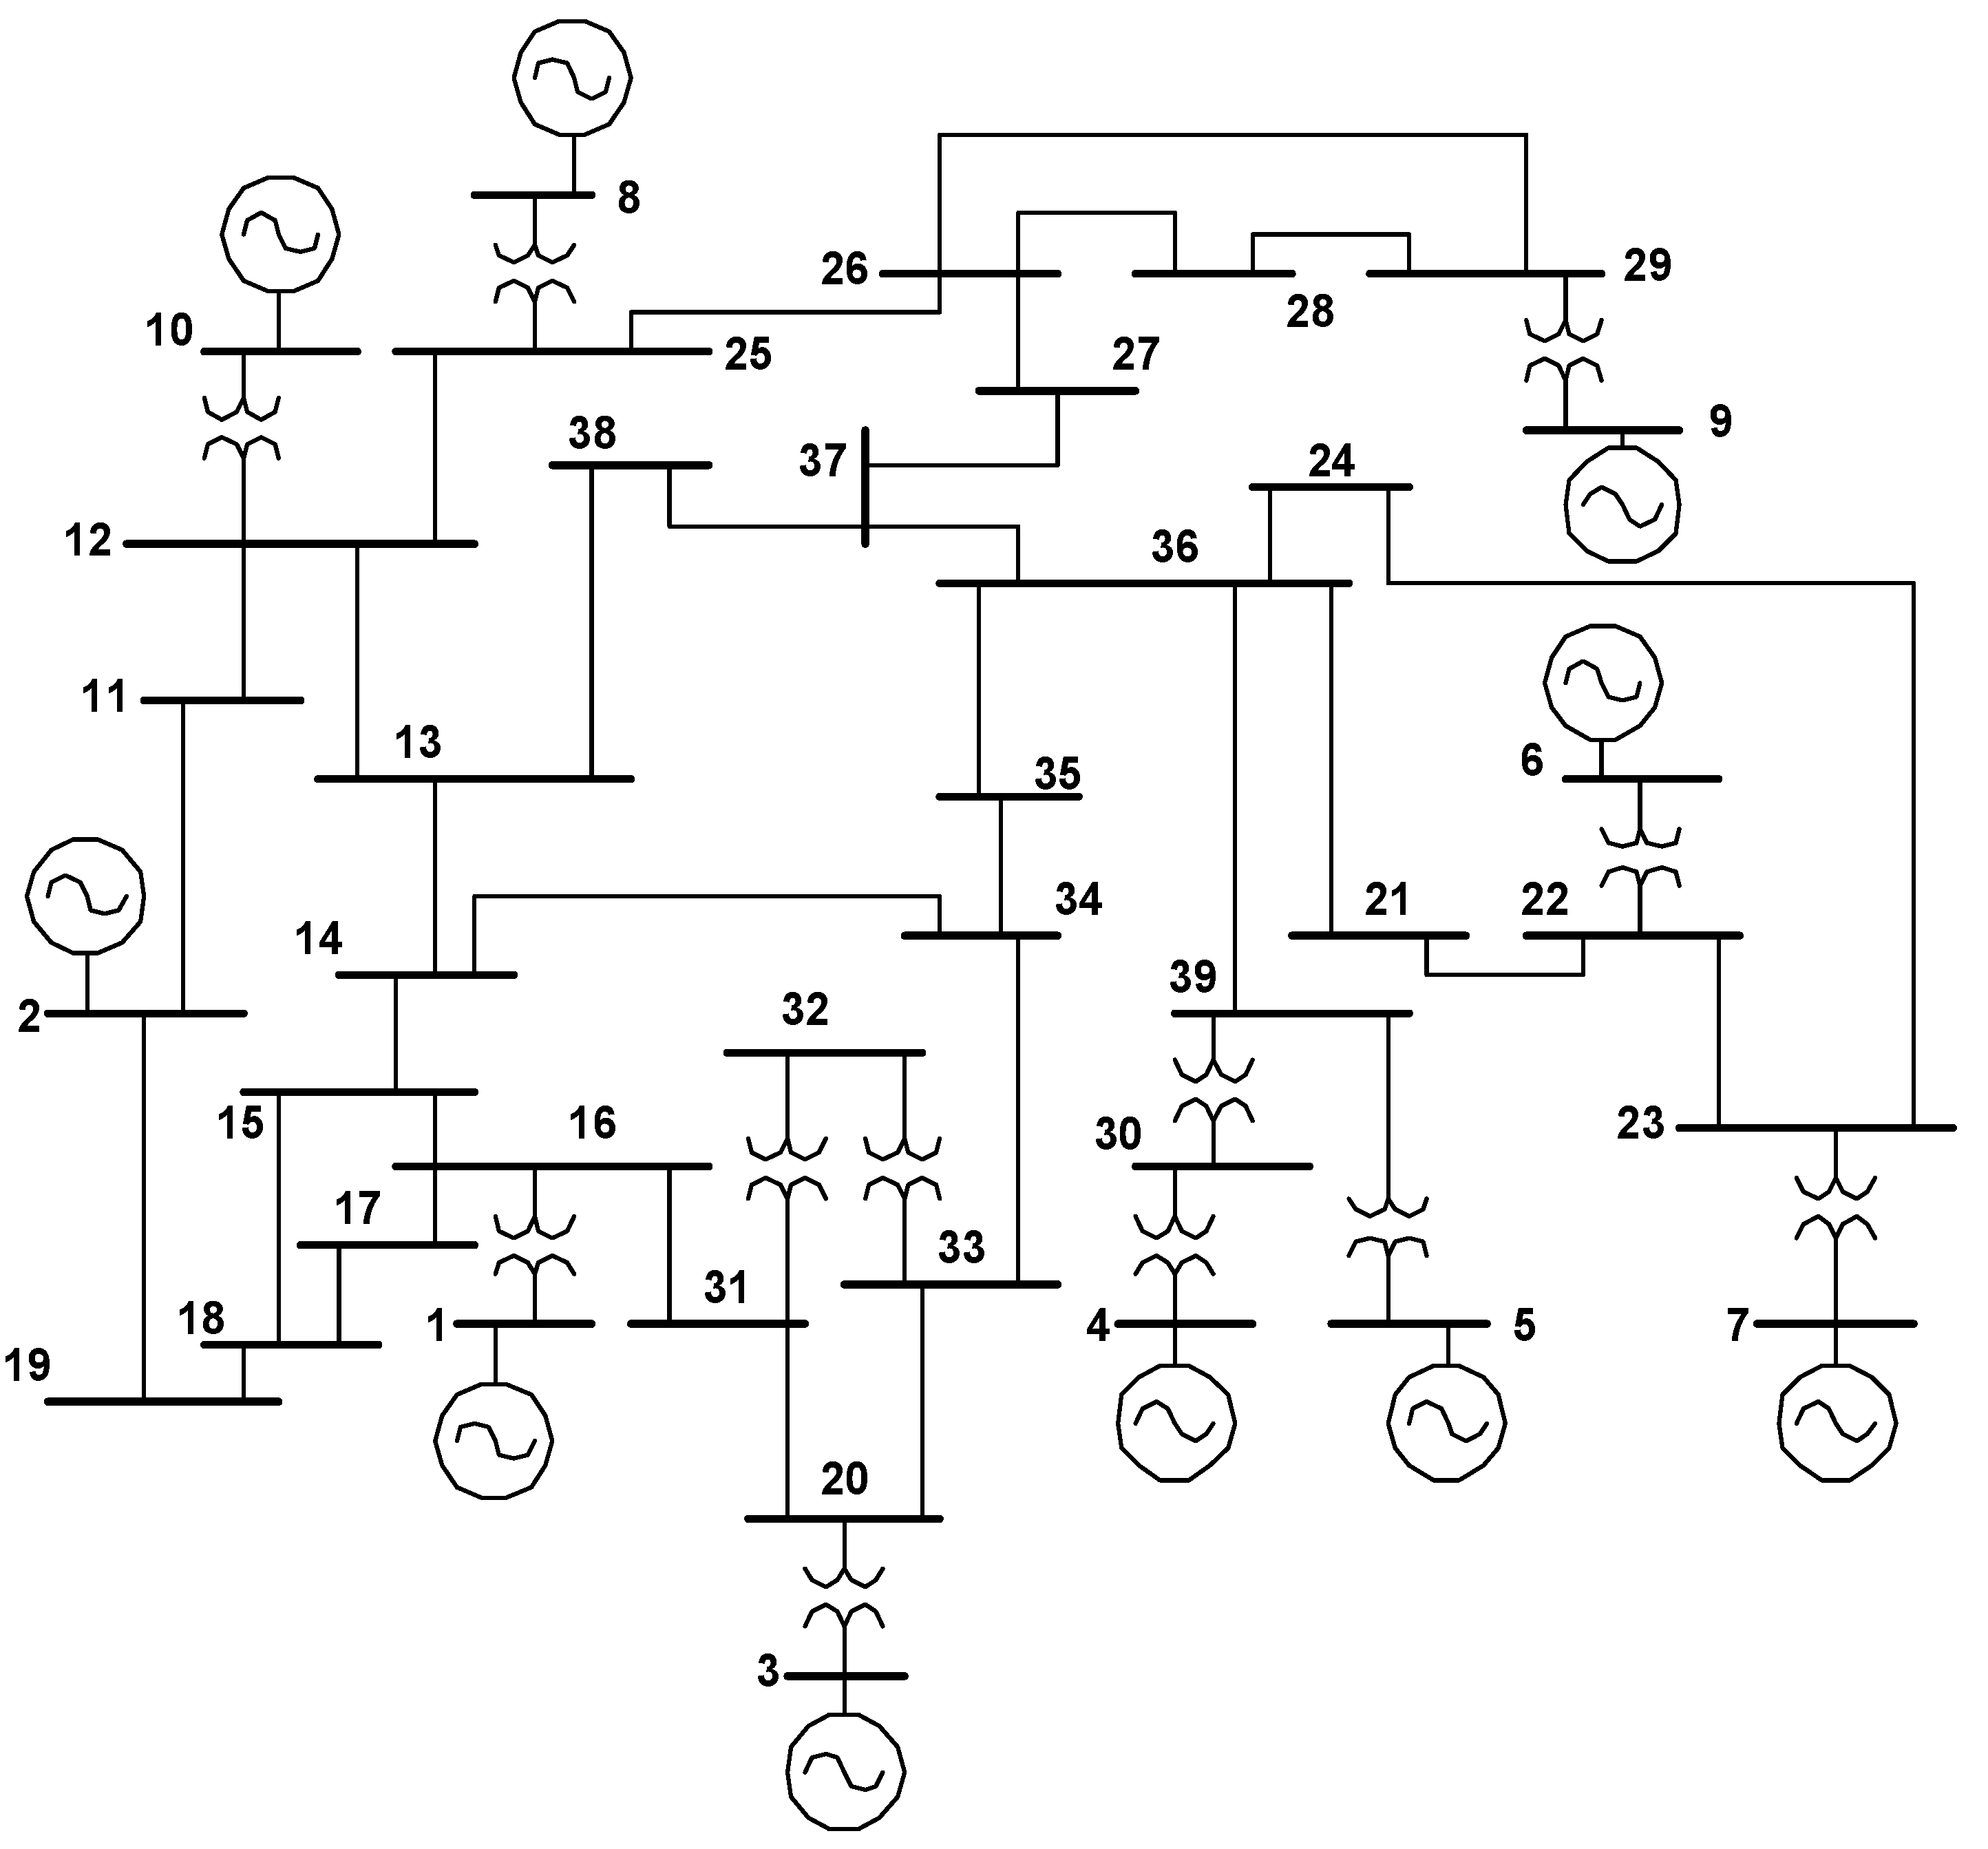
\includegraphics[width=0.47\textwidth]{img/ieee39bus}
\caption{
    The IEEE 39 bus example power transmission system.
}
\label{fig:example}
\end{figure}

%%%%%%%%%%%%%%%%%%%%%%%%%%%%%%%%%%%%%%%%

%\section{Discrete problem statement}
%
%We model a power grid during normal operations with the following linear dynamical system.
%\begin{equation}
%\begin{aligned}
%\label{sys:norm}
%\x_{t+1} &= A\x_t + B\uu_t + \epsilon
%\\
%\epsilon &\sim \normal{0}{Q^\epsilon}
%%\x_{t+1} &= (A + A^p_t)\x_t + B\uu_t + \epsilon ,~~~~~ \epsilon \sim \normal{0}{Q}
%\end{aligned}
%\end{equation}
%We assume that:
%(\emph{i})
%The matrices $A$ and $B$ are fixed in advance and known.
%These matrices depend on the physical characteristics of the power grid.
%(\emph{ii})
%The input $\uu_t$ is an unobserved control signal.
%This input represents normal industry and residential loads.
%(\emph{iii})
%The state variable $\x_t$ is fully observed at each iteration.
%The error term $\epsilon$ captures both observation and modeling error.
%
%%A load altering attack adds a new input term ${\uu_a}_t$.
%In a load altering attack, the attacker adds loads to the system in an attempt to destabilize it.
%We model these attacks with the following modified system.
%\begin{equation}
%\begin{aligned}
%\label{sys:attack1}
%\x_{t+1} &= A\x_t + B(\uu_t + \uu^{a}_t) + \epsilon
%\\
%\epsilon &\sim \normal{0}{Q^\epsilon}
%%\x_{t+1} &= (A + A^p_t)\x_t + B\uu_t + \epsilon ,~~~~~ \epsilon \sim \normal{0}{Q}
%\end{aligned}
%\end{equation}
%The input term $\uu^{a}_t$ captures the magnitude of the attack and is allowed to depend on time.
%When no attack is present, the term $\uu^a_t$ is zero, and the system above reduces to Equation \ref{sys:norm}.
%In a static load altering attack, the attack input $\uu^a_t$ remains a constant non-zero value throughout the attack.
%These attacks can introduce transients into the system,
%but they cannot destabilize the system.
%In a dynamic load altering attack, $\uu^a_t$ changes over time.
%Relatively small changes in $\uu^a_t$ can induce large, destabilizing changes in the system.
%This makes dynamic load altering attacks much more dangerous than their static counterparts.
%
%We consider the case where the attacker uses a proportional controller to dynamically determine the value of $\uu^a_t$.
%In this scheme, the attack load can be decomposed into $\uu^a_t = A^p\x_t + \uu^p_t$.
%The matrix $A^p_t$ represents the proportional gain of the attack and is allowed to vary arbitrarily over time;
%the input $\uu^p_t$ is assumed to remain constant throughout the attack (as in a static attack).
%Substituting into Equation \ref{sys:attack1} gives us our final system dynamics under attack.
%\begin{equation}
%\begin{aligned}
%\label{sys:orig}
%\x_{t+1} &= (A + A^p_t)\x_t + B(\uu_t + \uu^p_t) + \epsilon
%\\
%\epsilon &\sim \normal{0}{Q^\epsilon}
%%\x_{t+1} &= (A + A^p_t)\x_t + B\uu_t + \epsilon ,~~~~~ \epsilon \sim \normal{0}{Q}
%\end{aligned}
%\end{equation}
%The adversary manipulates $A^p_t$ and $\uu^p_t$ to add positive feedback to the system with the goal of destabilizing it.
%Our goal is to determine which states are subject to positive feedback so that we can take corrective action to restore stability.
%
%In particular, each row of the $A^p_t$ matrix corresponds to a bus in our power grid.
%During normal system operation, all entries of $A^p_t$ will be zero.
%During an attack, one or more entries of $A^p_t$ will be positive.
%Our goal is to identify the rows of $A^p_t$ containing positive values,
%as these rows correspond to system buses under attack.

%%%%%%%%%%%%%%%%%%%%%%%%%%%%%%%%%%%%%%%%

\section{Attack detection method}
Our attack detection procedure has two steps:
(\emph{i})
First we rewrite the system dynamics of Equation \ref{sys:attack2} in discrete time.
This lets us use the Unscented Kalman Filter to perform dual state estimation to simultaneously estimate the value of $K^{LG}$ and the system states.
(\emph{ii})
Then, we detect the presence of an attack by thresholding the estimate of $K^{LG}$.

%\subsection{Discretization}
We begin by discretizing Equation \ref{sys:attack2} as
\begin{equation} \label{eq:discrete}
\begin{aligned}
\x_{t+1} &= (\timestep A+sA^p_t+I)\x_t + \timestep B(\uu_t+\uu_t^p) + \epsilon
\\
\epsilon &\sim \normal{0}{Q^\epsilon}
\end{aligned}
\end{equation}
where $\timestep$ is a scalar that represents the length of a time step,
and $\epsilon$ is an error term capturing both our modeling and observation errors.
Recall that in the definition of $A^p_t$,
the $K^{LG}$ matrix is unknown and determined by the attacker;
all other elements are statically known.
Therefore, to estimate $A^p_t$, it is sufficient to estimate $K^{LG}$.

We can estimate $K^{LG}_t$ directly using dual state estimation.
In this technique, we augment the original dynamical system's state variables to also include the elements of $K^{LG}_t$.
The resulting augmented system is
\begin{equation}
\begin{aligned}
\begin{split}
\begin{pmatrix}
\x_{t+1} \\
\vectorize K^{LG}_{t+1}
\end{pmatrix}
&=
\begin{pmatrix}
sA + sA^p_t + I & 0 \\
0 & I
\end{pmatrix}
\begin{pmatrix}
\x_t \\
\vectorize K^{LG}_t
\end{pmatrix}
\\&~~~~~~~~~~+
\begin{pmatrix}
sB & 0\\
0 & I
\end{pmatrix}
\begin{pmatrix}
\uu_t + \uu_t^p + \uu_t^p \\
\uu^m_t
\end{pmatrix}
+
\begin{pmatrix}
\epsilon \\
\epsilon^m
\end{pmatrix}
\end{split}
\\
\epsilon \sim \normal{0}{Q^\epsilon}
~~~~~~~~~~~~~~~~~~~~~~~~~~~~~~~~~
\\
\epsilon^m\sim\normal{0}{Q^{\epsilon^m}}
~~~~~~~~~~~~~~~~~~~~~~~~~~~~~~
\end{aligned}
\label{sys:dualized}
\end{equation}
Here we have also introduced a new control input $\uu^m_t$ with error $\epsilon_m$.
The $\uu^m_t$ input vector is unobserved and controlled by the attacker.
The attacker uses $\uu^m_t$ to manipulate the $K^{LG}_t$ matrix (and hence the $A^p_t$ matrix).
The notation $\vectorize K^{LG}_t$ refers to the column vector constructed by stacking the columns of $K^{LG}_t$ on top of each other.
Note that this model is nonlinear because the $K_t^{LG}$ term appears in the definition of $A^p_t$.

To make the model easier to analyze, we introduce two simplifying assumptions.
First, we note that the control input $\uu^m_t$ is unobserved.
Therefore, we can model its contribution as a random error term.
In particular, we assume $\uu^m_t\sim\normal{0}{Q^m}$.
Second, we note that the typical attack involves only a few buses in the power grid.
So the matrix $K^{LG}_t$ will be highly structured.
We assume the rank-1 structure $K^{LG}_t=\kL_t\trans{\kG}_{t}$ where $\kL_{t}$ and $\kG_{t}$ are column vectors.
Under these assumptions, we can rewrite the dualized system described in Equation $\ref{sys:dualized}$ as
\begin{equation}
\begin{aligned}
\begin{pmatrix}
\x_{t+1} \\
\kL_{t+1} \\
\kG_{t+1} \\
\end{pmatrix}
&=
\begin{pmatrix}
sA + sA^p_t + I & 0 & 0\\
0 & I & 0\\
0 & 0 & I
\end{pmatrix}
\begin{pmatrix}
\x_t \\
\kL_{t} \\
\kG_{t} \\
\end{pmatrix}
+
%\begin{pmatrix}
%B \\
%I
%\end{pmatrix}
%\begin{pmatrix}
%\uu_t \\
%0
%\end{pmatrix}
%+
\begin{pmatrix}
\epsilon \\
\epsilon_1 \\
\epsilon_2
\end{pmatrix}
\\\epsilon &\sim \normal{0}{B(Q+Q^p)+Q^\epsilon}
\\\epsilon_1 &\sim\normal{0}{Q^m+Q^{\epsilon_1}}
\\\epsilon_2 &\sim\normal{0}{Q^m+Q^{\epsilon_2}}
\end{aligned}
\end{equation}
This system is still nonlinear, but it can be solved efficiently using the Unscented Kalman Filter (UKF) \cite{wan2000unscented}.

%When the model is partially linear (as in our case), we can use reduced sigma point filtering to improve speed with no loss in accuracy.
%\cite{morelande2006reduced}
%We can also improve speed by using a low rank approximation of the covariance matrix.
%\cite{padilla2010adaptive}

Now we describe our thresholding procedure.
Define the function $f_t(i) = \sum_{j=1}^n {K^{LG}_t}{(i,j)}$ to be the sum of the entries in the $i$th row of the $K^{LG}_t$ matrix.
This value is the total predicted attack happening on the $i$th bus in the power grid.
Define $\alpha_t=\argmax_i |f_t(i)|$ to be the bus we predict to be under the heaviest attack.
If $f_t(\alpha_t)$ is greater than some threshold $\tau$,
then we declare that the system is under attack at bus $\alpha_t$.
At this point we can take defensive measures such as isolating the bus from the system.

Given our estimated value of $A^p_t$, we can also estimate the sign and magnitude of the attack.
Let $\beta$ equal the maximum eigenvalue of $A + A^p_t$ minus the maximum eigenvalue of $A$.
That is, $\beta = \lVert A - A^p_t\rVert_2 - \lVert A \rVert_2$.
If $\beta$ is positive, then the attack added positive feedback into the system,
and if $\beta$ is negative, then the attack added negative feedback.
The size of $\beta$ is the amount of feedback added.

Calculating an eigendecomposition of $A+A^p_t$ can be expensive.
%In the following two special cases, we can bound $\beta$ without performing the decomposition.
%First, consider the case where all eigenvalues of $A^p_t$ are nonnegative.
We can avoid this calculation when all of the eigenvalues of $A^p_t$ are nonnegative.
This will occur, for example, when all of the entries of $A^p_t$ are positive.
In this case each eigenvalue of $A+A^p_t$ must be greater than or equal to the corresponding eigenvalue of $A$.
Furthermore, the maximum value of $\beta$ must be less than or equal to the maximum eigenvalue of $A^p_t$.
The rank-1 matrix $A^p_t=\kL_{t}\trans\kG_{t}$ is guaranteed to have at most one nonzero eigenvalue equal to $\trans\kL_{t}\kG_{t}$.
So this value is an upper bound on the magnitude of the attack.

%This method estimates both the \emph{sign} and \emph{magnitude} of an attack as follows.
%For each load bus attacked, there will be exactly one nonzero eigenvalue of the $A^p_t$ matrix.
%If the eigenvalues of the $A^p_t$ matrix are all nonnegative,
%then the eigenvalues of the matrix $A+A^p_t$ must be greater than or equal to the eigenvalues of $A$.
%This implies that the attack adds positive feedback into the system,
%and the system will become unstable if the maximum eigenvalue of $A+A^p_t$ is greater than 1.
%On the other hand, if the eigenvalues of the $A^p_t$ matrix are all nonpositive,
%then the eigenvalues of the matrix $A+A^p_t$ must be less than or equal to the eigenvalues of $A$.
%This implies that the attack adds negative feedback into the system.
%This negative feedback cannot cause an already stable system to destabilize;
%however, it could introduce transients that temporarily cause the system to exceed safe operating limits.
%In both cases, the trace of $A^p_t$ measures the amount of feedback (because the trace is the sum of the eigenvalues).
%When the set of eigenvalues of $A^p_t$ contains both positive and negative values,
%we can say nothing about relationship between the eigenvalues of $A+A^p_t$ and $A$ without also looking at their corresponding eigenvectors.

%In a typical scenario, the matrix $A^p_t$ will contain only a small number of nonzero entries.
%In the case of multiple attacks happening simultaneously,
%this value provides a one dimensional summary of the attack.

%\fixme{
    %It would be nice to place bounds on the accuracy of the estimate above.
    %I don't think this is possible for two reasons.
    %First, the UKF provides no guarantee on the accuracy of our $A^p_t$ estimates.
    %Second, even if we had the true $A^p_t$ value, the rank-1 approximation introduces potentially unbounded error.
    %We
%}

\section{Simulation}

We demonstrate the effectiveness of our method on two sets of simulated experiments.
The first sets of experiments show qualitatively the values of $f_t(i)$ in different scenarios.
These experiments demonstrate that our method is fast, robust to the number of attacks, and able to distinguish between positive and negative feedback.
The second experiments show quantitatively that our method accurately determines which bus is being attacked.

\subsection{Qualitative experiments}

All experiments in this section use a single randomly generated power grid with 100 generators and 100 load buses.
Standard methods for generating random graphs do not exhibit the topological and electrical properties of real world power grids \cite{hines2010topological}.
Therefore, we follow the \emph{clusterSmallWorld} procedure for generating the power grid \cite{wang2010generating}.
This procedure was designed specifically for modeling real world power grid structures.
An outline of the procedure is:
First generate a random number of ring shaped grids with fewer than 10 buses each;
Then randomly add connections between the buses until the average degree of each node is 4.
To ensure the stability of the resulting system,
we scale the $A$ matrix so that its maximum eigenvalue is no greater than 0.999.
This model generates realistically shaped power grids up to about 300 buses.
Once the grid has been generated, a load input ($\uu_t$) is sampled from a Gaussian process truncated so that values are always non-negative.

%This paper has a more complex method that is suitable for any infrastructure, not just powergrids.
%The idea is to model how infrastructure actually develops over time due to realworld constraints.
%The paper claims to accurately model nation-sized powergrids (more than 1000 buses).
%\cite{schultz2014random}

For the first experiment, we initiated an attack at time 0.1 seconds on a random bus $i$ getting feedback from bus $j$.
We model the attack by setting all the entries of $A^p_t$ to zero except for the entry in row $i$ and column $j$.
This entry is set so that the matrix $A+A^p_t$ has maximum eigenvalue 1.05,
ensuring that the attack destabilizes the system.
Figure $\ref{fig:destab}$ shows the results of running our UKF algorithm on the resulting system.
Our estimate of $A^p_t$ quickly converges to the correct value.

\begin{figure}
\begin{tabular}{cc}
\includegraphics[width=0.23\textwidth]{img/4-clusterSmallWorld-100-addUniform-400-spike-gaussian-Unobserved-rank1.eps}
&
\includegraphics[width=0.23\textwidth]{img/4-clusterSmallWorld-100-addUniform-400-spike-gaussian-Unobserved-rank1-ukf.eps}
\\
time (sec)
&
time (sec)
\end{tabular}
\caption{
    (\emph{left})
    The values of the system states $\x_t$ as a function of time.
    Each component of $\x_t$ is drawn as a separate line.
    Before the attack (at time 0.1 sec), all system variables are essentially zero.
    After the attack, the system is destabilized.
    (\emph{right})
    The values of $f_t(i)$ as a function of time.
    Each value of $i$ is drawn as a separate line.
    The true attack location is indicated in red.
    Our method quickly identifies the true location,
    and the estimate quickly converges to the true value.
    }
\label{fig:destab}
\end{figure}

Our next experiment shows how our predictions scale as a function of the number of attacks.
We repeat the same procedure as above, but add more nonzero entries to $A^p_t$.
The results of 3 and 5 nonzero entries are shown in Figure \ref{fig:numattacks}.
The rank-1 approximation of $K^L$ does fairly well even when the number of attacks increases.
This is surprising because the true $K^L$ matrix has rank equal to the number of attacks.

\begin{figure}
\begin{tabular}{cc}
   \includegraphics[width=0.23\textwidth]{img/4-clusterSmallWorld-100-addUniform-400-spike3-gaussian-Unobserved-rank1-ukf.eps}
&  \includegraphics[width=0.23\textwidth]{img/4-clusterSmallWorld-100-addUniform-400-spike5-gaussian-Unobserved-rank1-ukf.eps}
\\
time (sec)
&
time (sec)
\end{tabular}
\caption{
    The values of $f_t(i)$ with 3 attacks (left) and 5 attacks (right).
    As above, the attack locations are colored in red and non-attack locations are green.
    In both cases, our method quickly identifies that an attack occurs.
    In the case of 5 attacks, the rank-1 approximation of $A^p_t$ is not accurate enough to get a correct prediction of the values for all attack locations.
    Importantly, however, the value of $\alpha_t$ remains a correct attack location.
    If this bus is isolated, then the system will stabilize.
}
\label{fig:numattacks}
\end{figure}

%Then we apply 1, 3, or 5 attacks to the power grid on random buses.
%The results are shown in Figure \ref{fig:numattacks}.
%As expected, our rank-1 UKF has good accuracy when there is a single attack.
%Somewhat surprisingly, this method continues to work well even when there are multiple attacks.
%The displayed results are for only a single power grid, but the results are qualitatively similar on other power grids as well.

%\begin{figure*}
%\begin{tabular}{ccc}
%\\ 1 Attack
%&  3 Attacks
%&  5 Attacks
%%\\ \includegraphics[width=0.33\textwidth]{img/4-clusterSmallWorld-100-addUniform-400-spike-gaussian-Unobserved-rank1.eps}
%%&  \includegraphics[width=0.33\textwidth]{img/4-clusterSmallWorld-100-addUniform-400-spike3-gaussian-Unobserved-rank1.eps}
%%&  \includegraphics[width=0.33\textwidth]{img/4-clusterSmallWorld-100-addUniform-400-spike5-gaussian-Unobserved-rank1.eps}
%\\ \includegraphics[width=0.3\textwidth]{img/4-clusterSmallWorld-100-addUniform-400-spike-gaussian-Unobserved-rank1-ukf.eps}
%&  \includegraphics[width=0.3\textwidth]{img/4-clusterSmallWorld-100-addUniform-400-spike3-gaussian-Unobserved-rank1-ukf.eps}
%&  \includegraphics[width=0.3\textwidth]{img/4-clusterSmallWorld-100-addUniform-400-spike5-gaussian-Unobserved-rank1-ukf.eps}
%\end{tabular}
%\caption{
    %This figure shows the predicted attack levels on the same power grid (with 100 loads and 100 generators) in three different scenarios.
    %In each scenario, the attack happens at time 0.1 seconds.
    %The only difference between the scenarios is the number of attacks that occurred simulutaneously.
    %In each plot, the values of the estimated $A^p_t$ matrix are plotted over time.
    %Each line in the plot corresponds to a single entry in the matrix.
    %If an entry was actually attacked, then the corresponding line is colored red;
    %otherwise, the corresponding line is colored green.
    %In the left figure, only a single attack occurs.
    %Our algorithm is able to quickly identify the presence of an attack, which bus the attack occurred on, and the strength of the attack.
    %In the middle figure, three attacks occur simultaneously.
    %The algorithm is able to quickly identify the presence of an attack, but has slightly slower convergence to its steady state values.
    %In the right figure, five attacks occur simultaneously.
    %In this case, the algorithm is able to quickly identify the attack, but incorrectly predicts that some of the attacks are introducing negative feedback.
    %This is because our algorithm uses a rank 1 approximation of the $A^p_t$ matrix, but the true attack in this case requires a rank 5 matrix.
    %The closest rank 1 matrix to the attack matrix has negative numbers in the corresponding entries.
%}
%\label{fig:numattacks}
%\end{figure*}

Our last qualitative experiment shows that our UKF method can also detect negative feedback added to the power system.
We repeat the procedure of the first experiment,
but set the value of ${A^p_t}^{(i,j)}$ to $-10$.
Recall that negative values of the $A^p_t$ matrix correspond to negative feedback.
The results are shown in Figure \ref{fig:neg}.
Negative feedback does not destabilize the system,
yet we are still able to detect the feedback.
Previous methods could not differentiate between positive and negative feedback.

\begin{figure}
\begin{tabular}{cc}
\includegraphics[width=0.23\textwidth]{img/4-clusterSmallWorld-20-addUniform-20-spikeNeg-gaussian-Unobserved-rank1.eps}
&
\includegraphics[width=0.23\textwidth]{img/4-clusterSmallWorld-20-addUniform-20-spikeNeg-gaussian-Unobserved-rank1-ukf.eps}
\\
time (sec)
&
time (sec)
\end{tabular}
\caption{
    (\emph{left})
    The values of the system states $\x_t$ as a function of time as in Figure \ref{fig:destab}.
    The negative feedback is added at time 0.1 seconds.
    (\emph{right})
    The values of $f_t(i)$ as a function of time as in Figures \ref{fig:destab} and \ref{fig:numattacks}.
    The predicted value of the added location goes negative and is clearly separated from the rest.
    }
\label{fig:neg}
\end{figure}
\begin{figure}
\end{figure}

\subsection{Quantitative experiments}

For the experiments in this section, we randomly generated 20 different power grids following the same procedure as the previous section.
In each scenario, we use a single attack initiated at time 0.1 seconds.
The goal is to show that our method works on many realistic power grids and not just the special case demonstrated above.

A major strength of our method is that it has essentially no false positives.
We define a false positive to be the detection of an attack when no attack occurred (it does not matter if the value of $\alpha_t$ is correct).
When no attack is underway, the values of $A^p_t$ are typically less than $10^{-6}$.
When an attack is underway, the largest values of $A^p_t$ skyrocket to well above $10^{-1}$.
Therefore, it is easy to set the threshold $\tau$ to avoid false positives.

Next, we evaluate the accuracy of our method.
We define the accuracy at time point $t$ to be the fraction of $\alpha_t$ values that correctly predict the attacked bus.
Figure \ref{fig:accuracy} shows that the longer we wait to declare an attack occurs (i.e. the larger we set $\tau$), the higher our accuracy is.
If we are willing to wait two seconds after an attack begins before taking corrective action,
then we will essentially always be taking corrective action against the attacked bus.
In practice, two seconds is not enough time for an attack to have caused the state values $\x_t$ to exceed their safe operating values.

%The next important measure is the method's accuracy.
%That is, when we identify an attack
%First, we want to emphasize that our method has an essentially zero false positive rate.
%
%For the first experiment, we measured

\begin{figure}
\begin{tabular}{cc}
\begin{turn}{90}
~~~~~~~~~~~~~accuracy of $\alpha_t$
\end{turn}
&
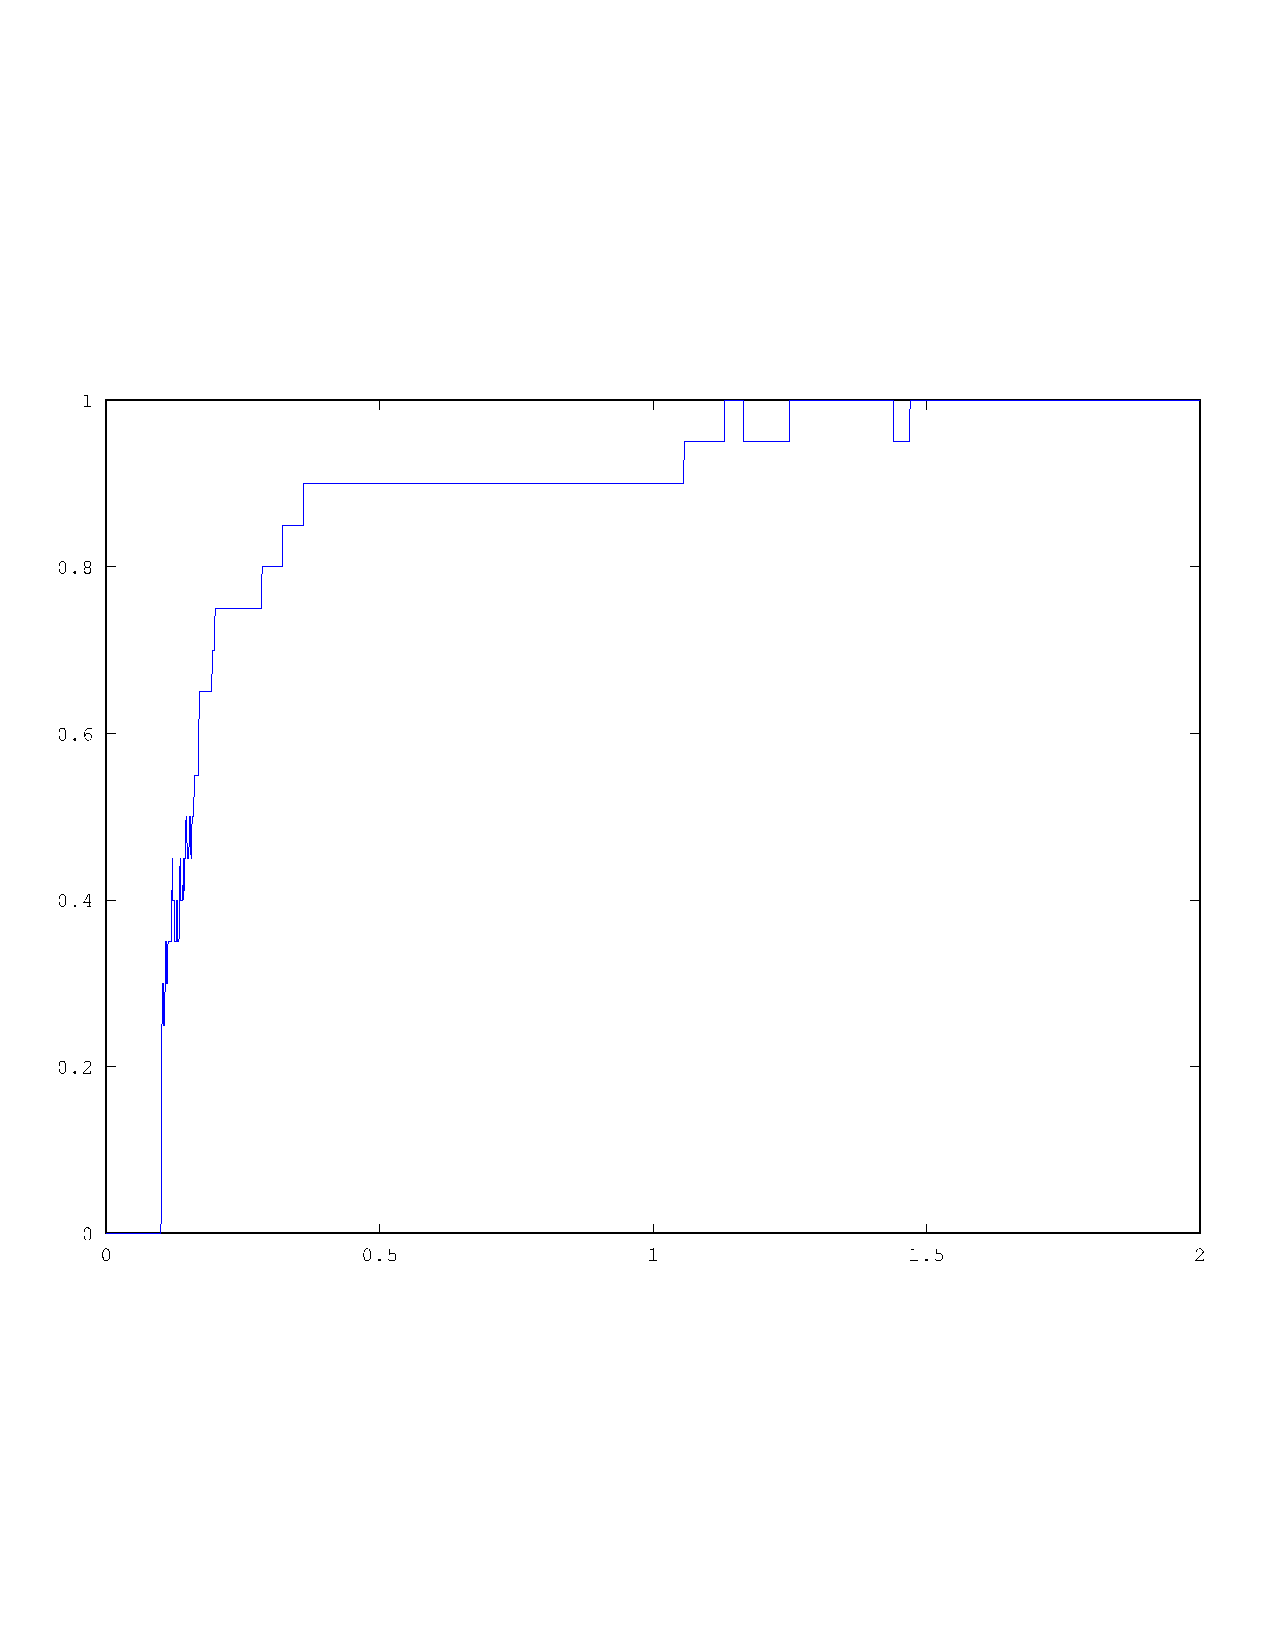
\includegraphics[width=0.4\textwidth, trim= 0 2in 0 2in, clip]{img/clusterSmallWorld-100-addUniform-400-spike-gaussian-Unobserved-rank1-ukf-fraction}
\\
& time
\end{tabular}
\caption{
    Immediately after the attack begins, $\alpha_t$ has modest accuracy.
    Within half a second, $\alpha_t$ has reached 90 percent accuracy.
    By two seconds, $\alpha_t$ is essentially 100 percent accurate.
}
\label{fig:accuracy}
\end{figure}

%\begin{figure}
%\begin{tabular}{cc}
%\begin{turn}{90}
%~~~~~~~~~~threshold
%\end{turn}
%&
%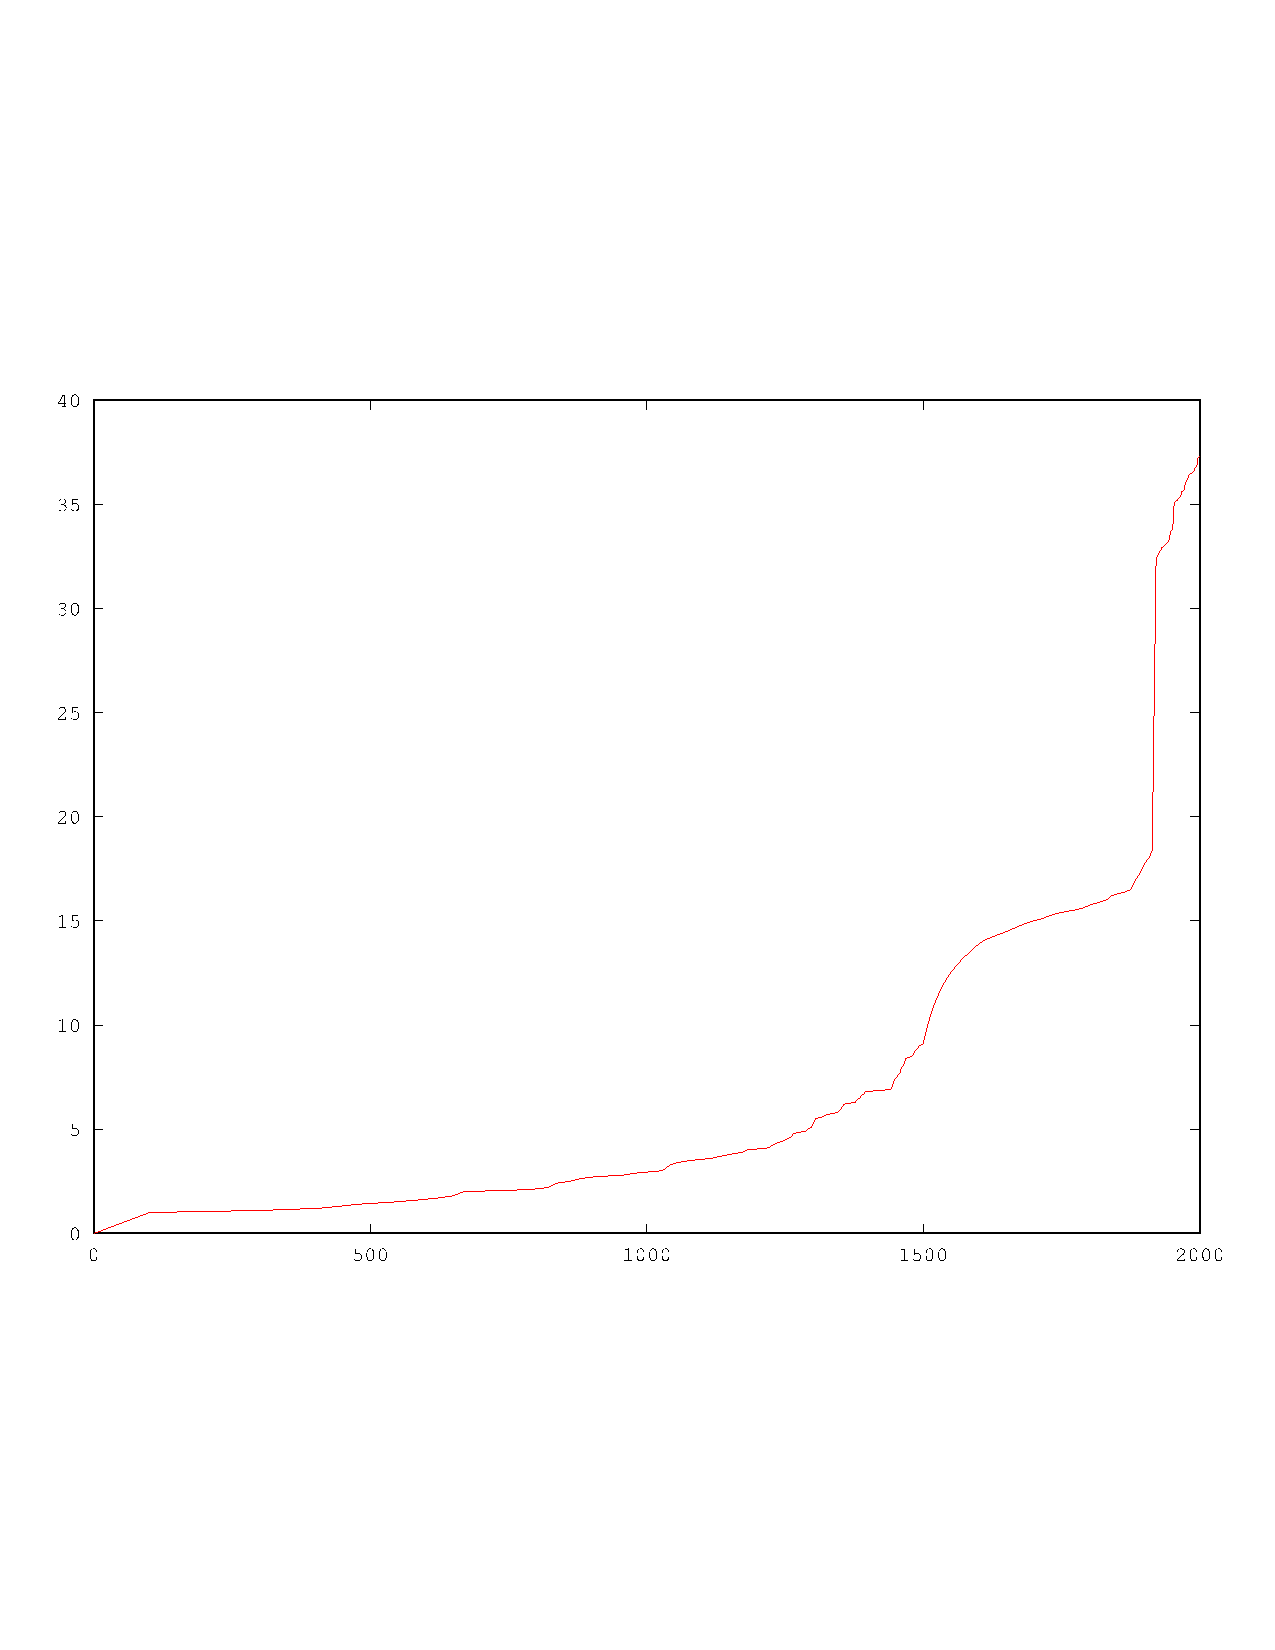
\includegraphics[width=0.4\textwidth, trim= 0 2in 0 2in, clip]{img/clusterSmallWorld-100-addUniform-400-spike-gaussian-Unobserved-rank1-ukf-thresholds}
%\\
%&
%time
%\end{tabular}
%\caption{
    %This plot shows the average time to first detection of an attack as a function of the threshold value.
%}
%\label{fig:threshold}
%\end{figure}

%%%%%%%%%%%%%%%%%%%%%%%%%%%%%%%%%%%%%%%%%%%%%%%%%%%%%%%%%%%%%%%%%%%%%%%%%%%%%%%%

\bibliographystyle{plain}
\bibliography{paper}
\end{document}
